\documentclass[aspectratio=169]{beamer}
\usetheme[block=fill]{metropolis}
\usepackage{tikz}
\usetikzlibrary{shapes.geometric, arrows.meta, positioning, calc}

\title{Building a Reproducible Scholarly Search Toolkit}
\subtitle{Episode 17: Command Line Interface (Argparse)}
\author{Scholar Search Kit}
\date{}

\begin{document}

\begin{frame}[plain]
  \titlepage
\end{frame}

\begin{frame}{Episode Goal}
  \begin{alertblock}{The Goal}
    Expose our Python API as a robust, user-friendly Command Line Interface using the standard \texttt{argparse} library.
  \end{alertblock}
  \vspace{0.5cm}
  Researchers shouldn't have to write Python scripts to use our tool. They should be able to type \texttt{scholar-search "AI in Healthcare" --provider openalex} in their terminal.
\end{frame}

\begin{frame}{CLI Architecture}
  \begin{center}
  \resizebox{0.6\linewidth}{!}{
  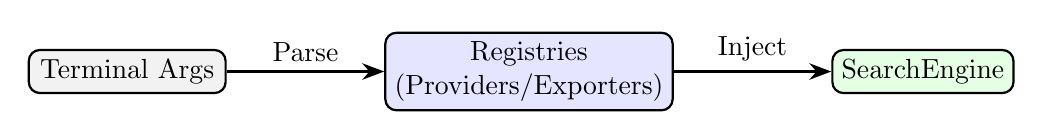
\begin{tikzpicture}[
      node distance=1.5cm and 2cm,
      cli/.style={rectangle, draw, thick, rounded corners, minimum width=2.5cm, align=center, fill=black!5},
      reg/.style={rectangle, draw, thick, rounded corners, minimum width=3cm, align=center, fill=blue!10},
      eng/.style={rectangle, draw, thick, rounded corners, minimum width=2cm, align=center, fill=green!10},
      arrow/.style={-{Stealth[scale=1.2]}, thick}
    ]
    
    \node[cli] (c) {Terminal Args};
    \node[reg, right=of c] (r) {Registries\\(Providers/Exporters)};
    \node[eng, right=of r] (e) {SearchEngine};
    
    \draw[arrow] (c) -- node[above] {Parse} (r);
    \draw[arrow] (r) -- node[above] {Inject} (e);
  \end{tikzpicture}
  }
  \end{center}
  \vspace{0.2cm}
  The CLI layer parses raw strings, looks up the requested classes in our Registries, instantiates the Engine, and presses "Run".
\end{frame}

\begin{frame}{Implementation: \texttt{argparse}}
  \begin{block}{Declarative Arguments}
    \texttt{argparse} automatically handles \texttt{--help} menus, type checking, and required vs optional flags.
  \end{block}
  
  \begin{itemize}
      \item \texttt{--query} (Required): The boolean search string.
      \item \texttt{--provider} (Optional, default: openalex): The backend source.
      \item \texttt{--format} (Optional, default: jsonl): The output format.
  \end{itemize}
\end{frame}

\begin{frame}{Handling Secrets}
  \begin{block}{API Keys}
    Never pass API keys via CLI arguments (they get logged in bash history).
  \end{block}
  
  \begin{itemize}
      \item We use \texttt{os.environ.get("CROSSREF\_API\_KEY")} so users can securely export their credentials in their profile.
  \end{itemize}
\end{frame}

\begin{frame}{Verification}
  \begin{alertblock}{Success Criteria}
    \begin{itemize}
        \item Running \texttt{python -m scholar\_search --help} prints a beautiful, well-documented menu.
        \item Passing an invalid provider name (e.g., \texttt{--provider fake}) raises a clean error message, not a Python stack trace.
    \end{itemize}
  \end{alertblock}
\end{frame}

\end{document}
